\chapter{Data and Models}
\label{chap:datamodels}

\section{Data}

This work addresses the question of machine learning integration by experimenting with documentary and descriptive data. Using field data will 1) reveal how current annotation methods affect the performance of NLP systems, 2) test the practicality of incorporating machine learning into the documentary and descriptive workflow, 3) demonstrate that IGT output of documentary and descriptive projects is sufficient to train machine learning models, and 4) enrich the selected data with the results of the experiments.
%A consensus among LDD practitioners is that more documented data is always better to support linguistic description or revitalization. This holds true for NLP as well: the more training data, the better the results. Yet, the combination of funding limitations and lack of integrated machine learning assistance means that the amount of interlinearized data that LDD projects is almost always less than what is collected and transcribed. 

The selected data corpora are representative of a range of typical documentary and descriptive projects. They consist of manually interlinearized glossed texts (IGT) from the nine under-documented and endangered languages summarized in Table \ref{tab:langs}.   

\bgroup
\def\arraystretch{1.25}
\begin{table}[h!]
    \begin{center}
    \begin{tabular}{lllll} 
    \textbf{Language} & \textbf{ISO} & \textbf{Family} & \textbf{Morphology} & \textbf{Status} \\
    \hline
    Alas & btz & Austronesian & Agglutinative & Stable \\
    %\hline
    Arapaho & arp & Algonquian & Polysynthetic & Severely Endangered  \\
    %\hline
    Lamkang & lmk & Sino-Tibetan & Agglutinative & Endangered/Stable   \\
    %\hline
    Lezgi & lez & Nakh-Daghestanian & Agglutinative & Vulnerable \\
    %\hline
    Manipuri & mni & Sino-Tibetan & Agglutinative & Vulnerable  \\
    %\hline
    Natügu & ntu & Austronesian & Agglutinative & Stable \\
    %\hline
    Southern Sierra Miwok & skd & Utian & Polysynthetic & Nearly Extinct \\ 
    Tsez & ddo & Nakh-Daghestanian & Agglutinative & Endangered \\
    Upper Tanana & tau & Athabaskan & Polysynthetic & Critically Endangered \\
	\end{tabular}
	\caption[Data]{Language name, ISO 639-3 code, language family, predominant morphological type, endangerment status.}
	\label{tab:langs}
\end{center}
\end{table}


\subsection{Languages} 

The selected languages are spoken across five continents.
%, with populations of speakers ranging from a few hundred to about two million. 
Published linguistic resources are limited, meaning all these languages are under-documented. Information about speaker population and endangerment status was retrieved from the \emph{Ethnologue} \citep{eberhard_ethnologue:2020} and \emph{Catalogue of Endangered Languages} \citep{elcat_2020}.
%UNESCO’s \underline{Atlas of Endangered Languages} \citep{moseley_atlas_2010}.

\paragraph{Alas}
[btz] (Alas-Kluet, Batak Alas, Batak Alas-Kluet) belongs to the Malayo-Polynesian branch of the Austronesian family. It is spoken by 200,000 people on the Indonesian island of Sumatra. It is unclear if the three dialects (Alas, Kluet, and Singkil) constitute one language. The selected corpus is from the Alas dialect.  Its morphology features reduplication, infixation, and circumfixation. The corpus consists of 12 transcribed texts and one set of elicited sentences written with the Indonesian orthography. 
% Although the data was processed in FLEx, it is not surface segmented. I"m not sure how/why this is.

\paragraph{Arapaho}
is an Algonquian language spoken by about 200 people in Wyoming, USA, but spoken fluently by less than 50. It is highly agglutinating and polysynthetic, with the verb carrying the heaviest morphological load \citep{cowell_arapaho_2008}. This includes noun incorporation, where special forms of certain nouns become part of the verb. The corpus contains narratives and conversation from the 1880s until the present day, including a few religious texts that are translations from English. The corpus is in the popular Arapaho orthography. Much of the data is available through the Endangered Languages Archive\footnote{\url{https://elar.soas.ac.uk/Collection/MPI189644}} or the Center for the Study of Indigenous Languages of the West\footnote{\url{https://www.colorado.edu/center/csilw/arapaho-language-archives}} at the University of Colorado.

\paragraph{Lamkang} 
is a Northern Kuki-Chin language in the Tibeto-Burman family. Depending on the primary source of population numbers, speakers are estimated between 4 to 10 thousand people. Speakers live primarily in Manipur, India but also in Burma \cite{lamkang_2007}. Its endangerment status is also not clear. It tends toward agglutination with many stem-stem patterns to signal syntactic categories. Many morphemes are written as separate words in the corpus. There is limited literacy material available. The corpus is at the Computational Resources for South Asian Languages (CoRSAL) digital archive at the University of North Texas.\footnote{\url{https://digital.library.unt.edu/explore/collections/SAALT/}}

\paragraph{Lezgi} 
(Lezgian) belongs to the Lezgic branch of the Nakh-Daghestanian (Northeast Caucasian) family. It is spoken by over 400,000 speakers in Russia and Azerbaijan. Lezgi is an highly agglutinative language with overwhelmingly suffixing morphology. The corpus contains oral texts in the endangered Qusar dialect of Azerbaijan. This dialect differs from the standard written dialect in a few ways, such as a locative case suffix borrowed from Azerbaijani which is used alongside the native inessive case suffix with the same meaning. The texts are transcribed into the language's Cyrillic orthography and is the only corpus used in this research that is transcribed in a non-Latin alphabet. The corpus is being deposited at SIL Language and Culture Archives.

\paragraph{Manipuri} 
(Meitei, Meetei) belongs to the Tibeto-Burman branch of the Sino-Tibetan family. It is spoken by nearly two million people, primarily in the state of Manipur, and is one of India's official languages. It has nevertheless been classified as vulnerable to extinction by UNESCO. It is a tonal language and has weakly suffixing, agglutinative morphology \citep{Chelliah-1997}. It is the only Tibeto-Burman language in India with its own script, but the corpus was transcribed with the international Phonetic Alphabet (IPA). The corpus is available through the Computational Resources for South Asian Languages (CoRSAL) digital archive.\footnote{\url{https://digital.library.unt.edu/explore/collections/MDR/}}

\paragraph{Natügu}
belongs to the Reefs-Santa Cruz group in the Austronesian family. It is spoken by about 4,000 people in the Temotu Province of the Solomon Islands. It has a mainly agglutinative morphology with complex verb structures \citep{naess_ntu_2008}. The corpus contains transcribed narratives and a large written text. The data is available through SIL Language and Culture Archives\footnote{\url{https://www.sil.org/resources/search/language/ntu}} or is being deposited at the Pacific and Regional Archive for Digital Sources in Endangered Cultures (PARADISEC).

\paragraph{Southern Sierra Miwok} 
is a member of the Utian (Miwok-Costanoan) family of central California (USA) \citep{broadbent_southern_1964}. There are likely no fully fluent native speakers remaining. Verbs inflect for both subjects and objects and have fairly complex derivational morphology with extensive allomorphy. The corpus consists of narratives and conversation from the early 1900s to the 1980s, and is archived and available upon request from the Center for the Study of Indigenous Languages at the University of Colorado.\footnote{\url{https://www.colorado.edu/center/csilw/arapaho-language-archives}}

\paragraph{Tsez}
(Dido) belongs the Tsez-Hinukh branch of the Nakh-Daghestanian family. It is spoken by about 12,500 speakers in Daghestan, Russia. It has a rich agglutinative, suffixing morphology. The corpus is made up of folklore and is part of the Tsez Annotated Corpus Project \citep{abdulaev-tsezcorpus-2010}. It is available online\footnote{\url{https://tsezacp.clld.org/}} stored and preserved by Zenodo.org.

\paragraph{Upper Tanana}
(Nabesna) belongs to the Alaskan sub-group of the Northern Dene (Athabaskan) family. Although it is one of the official languages of Alaska and has been taught in a Canadian school, it is critically endangered, with barely 50 adult speakers in the eastern interior of Alaska (USA) and the Yukon Territory (Canada) \citep{lovick_grammar_2020}. Its complex morphology features non-continuous lexical, derivational, and inflectional prefixes on verbs. The corpus was collected in 2006-2019 in Alaska; most speakers represented the Tetlin and Northway dialects. 
%Two annotators did most of the interlinearization with small contributions from 2 or 3 others. 
The primary data (recordings, transcripts) is preserved at the Alaska Native Language Archive.\footnote{\url{https://www.uaf.edu/anla/}}



\subsection{Corpora}

%Publicly available structured resources such as UniMorph and Wiktionary are convenient sources for minority language data. They allow community contribution of material that can support the development of NLP and Human Language Technology.

The data was selected primarily to represent a range of “typical” outputs by documentary and descriptive projects. Less effort was made to represent typological structures, geographic areas, or a range of language families, although some attempt was made to keep an even distribution of morphological types. No attempt was made to include fusional morphology since it is already well-represented in high-resource languages. The texts are mostly narratives that were transcribed from recorded speech. Since the sample of languages is small, the analyses in this work avoid sweeping claims that depend on linguistic typology or discourse genre. 
The corpora were generously shared in the form of backup XML or CSV files. The rights holders gave informed consent to use the data research purposes. 
%The data providers also agreed to be available to answer questions about their projects and conduct error analysis when necessary.

Even though most of the corpora resulted from many years of work, they still stand as prime examples of the annotation bottleneck in language documentation and description. More data was recorded and transcribed than could be interlinearized within the project's budget. Each project's unique priorities and workflow resulted in different proportions of fully segmented and glossed data, as shown in Table \ref{tab:dissdata}.
Only the Arapaho and Tsez corpora can be considered completed (though missing annotations were found in both during preprocessing). 


\begin{table*}
    \centering
    \begin{tabular}{l|r|r|rc|rc|rc}
         \textbf{Language} & \textbf{Tokens} & \textbf{Inflected} & \multicolumn{2}{c|}{\textbf{Segmented}} & \multicolumn{2}{c|}{\textbf{Glossed}} & \multicolumn{2}{c}{\textbf{POS-tagged}} \\
         \hline
         Alas & 4.5k  & 412 & 3,840 & 86\% & 3,775 & 83\% & 3,845  & 86\% \\
         % 4462 btz raw number of tokens 
         % segmented and glossed: 3775/4462 = 0.846
         % segmented in both ways with no editing: 3715/4462 = 0.832
         % surf segmented: 3840/4462 = .860
         % canonically segmented: 3840
         % glossed: 3775
         % translated: 302/303
         % POS tagged: 3845/4462 = .861
         %inflected: 412
         \hline
         Arapaho & 300k &  56,922 & 202,760 & 69\%  & 201,915 & 68\% & 0  & 0\%  \\
         % 294,774 arp actual number of tokens
         \hline
         Lamkang & 101k & n/a & 49,699 & 49\%  & 50,252 & 50\% & 46,557 & 46\% \\
         % segmented & glossed: 50252/101005 = 0.497
         % segmented in both ways with no editing: 43814/101005 = .433
         % surf segmented: 60667
         % canonically segmented: 49699/101005 = .492
         % glossed: 50252
         % translated: 8629/8640 = 0.998
         % POS tagged: 46557/101005 = .460
         \hline
         Lezgi & 14k & 588 & 13,625  & 98\%  & 13,353  &  94\% & 13,636 & 96\%  \\
        % 14175 lez actual number of tokens
        % segmented & glossed: 13353/14175 = 0.942
         % segmented in both ways with no editing: 12797/14175 = 0.902
         % surf segmented: 13943
         % canonically segmented: 13625/14175 = .983
         % glossed: 13353
         % translated: 1531/1532
         % POS tagged: 13636/14175 = .961
         \hline
         Manipuri & 12k  & 2,192 & 11,907 & 98\%  & 11,907 & 98\% & 2,067 & 17\% \\
        % 12139 mni actual number of tokens 
        % segmented & glossed: 11907/12139 = 0.980
         % segmented in both ways with no editing: 10635/12139 = 0.876
         % surf segmented: 12187
         % canonically segmented:  11908/12139 = 
         % glossed: 11907
         % translated: 1784/1785
         % POS tagged: 2067/12139 = .170
         \hline
         Natügu & 16.5k & 1,646 & 14,136 & 86\%  & 13,925 &  84\% & 10,994 & 66\% \\
        % 16520 ntu actual number of tokens 
        % segmented in both ways with no editing: 12435/16520 = 0.752
         % MWE seg & glossed: 13924/16520 = 0.842
         % surf segmented: 14577
         % canonically segmented:  14136/16520 = .855
         % glossed: 13925
         % translated: 1541/1542
         % POS tagged: 10994/16520 = .665
         \hline
         Sierra Miwok & 10k  & n/a & 7,422 & 72\% & 7,413 & 72\% & 0  & 0\% \\
         \hline
         Tsez & 53k & 7,315 & 53,025 & 100\% & 53,025 & 100\% & 0  & 0\%  \\
         %lines: 4949
         %raw tokens: 53145
         \hline
         Upper Tanana & 17.5k & n/a & 11,930 & 68\% & 11,867 & 67\% & 11,198 & 64\% 
    \end{tabular}
    \caption[Data Statistics]{Tokens include multiple word expressions (when parsed as such) as single tokens and ignores tagged English words, proper nouns, digits, and punctuation. Inflected refers to the number of unique inflected forms that can be used to train the inflection task. The percentage and total number of tokens that are segmented or glossed are shown.  The segmentation and glossing task trains on both. The inflection task needs only glossed tokens.}
    \label{tab:dissdata}
\end{table*}

%\begin{table}
%    \centering
%    \begin{tabular}{lccc}
%        \textbf{Language} & \textbf{Seg/Gloss} & \textbf{Translated} & \textbf{Ratio}\\
%        \hline
%        Alas & 75\% & 100\% & 3:4 \\
%        \hline
%        Arapaho &  &  \\
%        \hline
%        Lezgi &  &  \\
%        \hline
%        Manipuri &  &  \\
%        \hline
%        Natügu &  &  \\
%        \hline
%        Tsez & 100\% & 100\% & 1:1 \\
%    \end{tabular}
%    \caption[Proportions of Completed Interlinear Lines]{The percentage of lines in each corpus that were completely segmented and glossed (Seg/Gloss) and the percentage that was translated.}
%    \label{tab:proportion}
%\end{table}

Each corpus required preprocessing because of errors, typos, changing analyses, or variable formatting. Even projects that employed the same software tool had variable formatting. For example, both Natugu and Bahasa Alas have circumfixing, but in one corpus the prefixed part was labeled as a circumfix and the suffixed part as a suffix, while the other corpus took the opposite approach. 
%Other issues arose from the variety of fonts for models that only accept ASCII characters. 

Gold standard data for training and testing was produced by filtering incomplete annotations. Only tokens that were completely segmented and glossed, and only sentences that were translated are included in the gold standard for the relevant experiments. The resulting data sizes are given in Table \ref{tab:data}.

The projects that produced the corpora spent different amounts of time on interlinearization, had different short-term goals, and varied by team size, team members' education or linguistic training. For example, the Alas corpus was produced in a matter of months while the Arapaho and Natügu corpora were produced by projects that have extended over many years. These two corpora, as well as the Tsez corpus, were annotated by teams with multiple linguists and native speakers. In contrast, the projects that produced the Alas corpus and most of the Lezgi corpus had one linguist and one or two native speaker annotators. The smaller, shorter projects were usually not able to provide as much training to annotators. Most projects were undertaken with the primary goal of documenting and describing the language, but the shorter-term goal of the Alas project is to support literacy efforts while most of the work on the Lezgi corpus was done to support an MA thesis on verbs. These factors are reflected in the quality of the interlinearization. For example, in the Lezgi corpus only verbs were consistently annotated by a trained linguist. The rest was annotated by a native speaker with minimal linguistic training and, therefore, contains more errors and inconsistencies. 

The analyses of results in this research often refers to issues that arise from the annotation process. 
Variation in the IGT corpora is problematic for comparative analysis. The IGT vary in size and annotation quality. The issues due to size become clear in most cases when comparing results, and the answer from consensus would be that more data is always better. Some of the quality factors are brought to focus in the error analyses and discussions.
%The research assumes certain issues are more significant than others. 
The less significant factors, such as typos in glosses and inconsistent morpheme segmentation, are ignored or handled during preprocessing. Some of the more significant issues, such as different segmentation strategies (surface vs. canonical) and varying proportions of POS tagged data is addressed directly in this work.


\section{Models}
\label{sec:models}

The experiments use supervised machine learning systems. All implement models have achieved state-of-the-art NLP results in low-resource settings. They include the feature-based Conditional Random Fields and Support Vector Machine, and the neural LSTM-based encoder-decoder and Transformer. All models have been trained on an NVIDIA GP102 [TITAN Xp] GPU unless otherwise mentioned.
% Some of Ling's stuff was trained on the the research computing infrastructure.
%The models will be trained for three tasks: 1) morpheme segmentation and glossing, 2) translation, and 3) inflectional paradigm induction.

\paragraph{Conditional Random Fields (CRF).} The best performing non-neural model for sequence prediction such as morpheme segmentation and glossing is Conditional Random Fields (CRF) \citep{lafferty_conditional_2001,muller_efficient_2013,ruokolainen_comparative_2016}. The CRF is a sequence classifier that considers the whole sequence of symbols (words, letters, glosses, etc.) when making an individual prediction. It tries to optimize the probability of a complete sequence of labels, where each individual label is given a conditional probability based on the previous label and an arbitrary number of surrounding inputs. %\mans{This is tricky to word correctly. A CRF tries to optimize the probability of a complete sequence labeling, where each individual label gets a conditional probability based on the previous label and arbitrary surrounding inputs. Let's make sure to revisit this at some point.} 
The CRF has performed well on boundary detection (segmentation) and labeling (glossing). 

This work implements a linear-chain CRF \citep{lafferty_conditional_2001} with \textit{CRFsuite} \citep{okazaki2007} and its Python API.\footnote{\url{https://python-crfsuite.readthedocs.io/en/latest/}} The training parameters uses L-BFGS optimization \cite{liu1989} and Elastic Net regularization, i.e. a linear combination of $L_1$ and $L_2$ penalties. Maximum iterations for early stopping are set at 50.


\begin{figure}
    \centering
    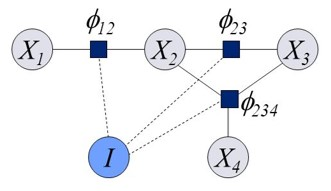
\includegraphics[width=6cm]{figs/CRF.jpg}
    \caption[Conditional Random Fields]{Conditional Random Fields sequence classifier.\footnote{source: www.slideplayer.com/slide/9361527}}
    \label{fig:CRF}
\end{figure}


%CRF learn to predict sequences with the help of pre-chosen features extracted from the data. Logistic regression allows the predictions to be generalized from arbitrary and possibly dependent features \citep{ruokolainen_supervised_2013}.  
%According to Ruokolainen et al. \cite{ruokolainen_comparative_2016}, discriminative models, compared to generative models, generalize better and optimize boundary detection.
%The strength of a discriminative model such as the CRF lies in its ability to examine more features than the ones extracted for the current symbol. 
%It assigns arbitrary weights to the features during training. 

For the CRF (Fig. \ref{fig:CRF}), predictions are scored over the whole sequence and then transformed into a probability distribution. The conditional distribution of the output sequence {\bf y}, given the input {\bf x} can be modeled as

\begin{equation}
p(\vect{y}|\vect{x}) = \frac{1}{Z} \textrm{exp}\Big(\sum_{i=1}^n\phi(y_{i-1}, y_i,\vect{x},i)\Big)
\end{equation}

\noindent where $\phi$ is the feature extraction function which can be expressed through a sum of $k$ individual component functions

\begin{equation}
\phi(y_{i-1}, y_i,\vect{x},i) = \sum_k w_k f_k(y_{i-1}, y_i,\vect{x},i)
\end{equation}

\noindent Here, $Z$ is the ``partition function'' which normalizes the expression to a proper distribution over all possible taggings given an input. 

\paragraph{Support Vector Machine (SVM).} Experiments with segmentation and glossing will compare sequential and joint methods. One sequential methods first segments morphemes with the CRF and then glosses them with a Support Vector Machine (SVM) \citep{svm_cortes}. The SVM will label only after segmenting is done by the CRF, using its own feature scheme. The SVM will be implemented as a multi-class linear SVM using the LIBLINEAR package \citep{fan2008}. It creates hyperplanes to separate the data into classes. The optimal hyperplane is found by maximizing the margin between the closest data points in each class, as illustrated in Figure \ref{fig:SVM}. These data points are the support vectors. Like CRF, the SVM learns from extracted features.

%\Mans{You should make clear that we used an SVM as a labeler after the segmentation was done, using some feature scheme. Otherwise a reader will be confused as to how you an SVM as a sequence labeler (possible, but not normally done) vs. a CRF which is inherently a sequence labeler.}

\begin{figure}[b]
    \centering
    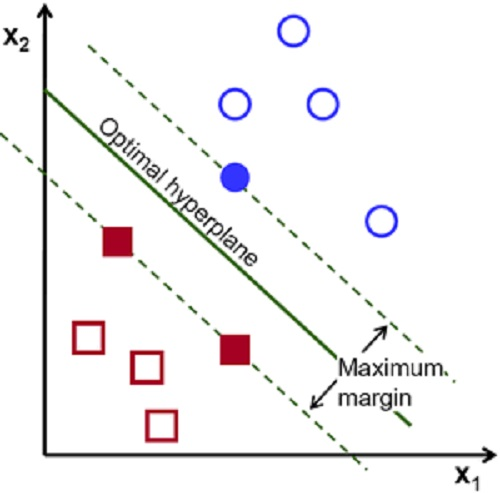
\includegraphics[width=5cm]{figs/SVM1.jpg}
    \caption[Support Vector Machine]{A Support Vector Machine (SVM).\footnote{source: www.aitrends.com/ai-insider/support-vector-machines-svm-ai-self-driving-cars/}}
    \label{fig:SVM}
\end{figure}

\paragraph{Transformer.} 
The primary model used in this work is the neural transformer model \citep{vaswani_attention_2017} in all three studies. The Transformer is a state-of-the-art neural model architecture for morphological tasks \citep{vylomova2020sigmorphon} that has achieved promising results for NLP in low-resource languages \citep{abbott_towards_2018,Martinus2019AFO}. 
%Like most neural models, the transformer’s main drawback in low-resource settings is its sensitivity to hyper-parameters.
It is a encoder-decoder model that uses Attention to boost speed and performance, as illustrated in Figure \ref{fig:transformer}. Attention allows the model to look at different elements in the sequence to help it encode/decode a given element before feeding it to the next encoder. The decoder has an additional attention layer that allows it to focus not only on the input sentence but also on the output sequence up to the element it is decoding. The order of elements in the sequence is represented as an embedding which is input to the encoder/decoder. 
%The standard Transformer encoder consists of identical layers, each of which has a multi-headed self-attention layer, and  one feed-forward layer. A residual connection is around two sub-layers, followed by layer normalization.

\begin{figure}[t]
    \centering
    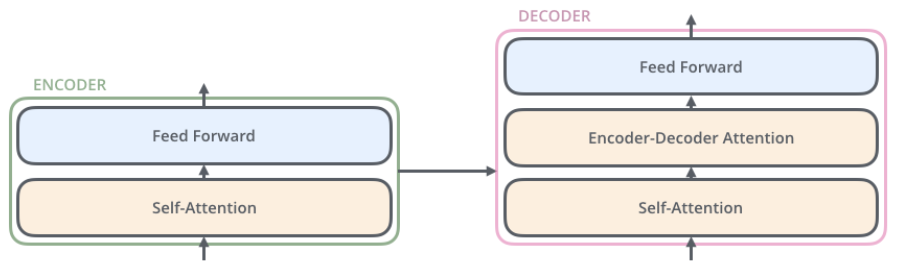
\includegraphics[width=10cm]{figs/Transformer_simplified.png}
    \caption[Transformer]{The Transformer encoder.\footnote{source: http://jalammar.github.io/illustrated-transformer/}}
    \label{fig:transformer}
\end{figure}

In all cases, the model is implemented with the Fairseq\footnote{\url{https://fairseq.readthedocs.io/en/latest/}} toolkit \citep{ott2019fairseq} with modifications and code \citep{wu_applying_2020} that have been successful with character-level transduction for morphology learning in low-resource settings. The parameters employed were $N=4$ layers for the encoder and the decoder, each with 4 self-attention heads. The embedding size for the encoder and decoder is 256, and the hidden layer size is 1024. A dropout rate of 0.3 for encoding and beam search with a width of 5 at decoding time was used. The adam algorithm \citep{kingma2014adam} ($\beta_1 = 0.9$, $\beta_2 = 0.98$) was used to optimize the cross entropy loss with label smoothing \citep{szegedy2016rethinking} of 0.1. 
%\footnote{4 encoder-decoder layers, 4 self-attention heads, 256 embedding size, 1024 hidden size of feed-forward layer, layer normalization before self-attention, decoding left-to-right in a greedy fashion} 



\paragraph{LSTM encoder-decoder.} In Chapter \ref{chap:IGT2P} a LSTM sequence-to-sequence model with exact hard monotonic attention for character-level transduction is used \citep{wu-cotterell-2019-exact}. This model is serves as baseline to compare the newer transformer model. 
